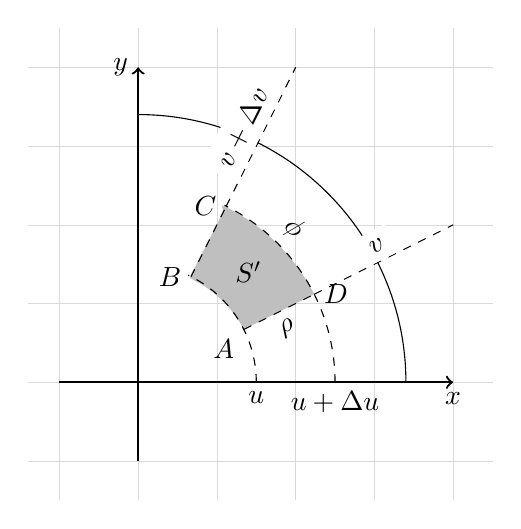
\begin{tikzpicture}
  \draw[very thin, gray!30, step = 1cm] (-1.4, -1.5) grid (4.5, 4.5);
  \draw (3.4, 0) arc (0 : 90 : 3.4cm);

  \draw[thick] [->] (-1, 0) -- (4, 0) node[below] {\(x\)};
  \draw[thick] [->] (0, -1) -- (0, 4) node[below, left] {\(y\)};
  
  %% нет, мне не стыдно
  \fill[lightgray] (1.342, 0.671) arc (28 : 65 : 1.5cm)
    -- (1.118, 2.236)
    -- cycle;
  \fill[lightgray] (2.236, 1.118) arc (27 : 65 : 2.5cm)
    -- (1.342, 0.671)
    -- cycle;

  \draw[dashed] (1.5, 0) arc (0 : 65 : 1.5cm);
  \draw[dashed] (2.5, 0) arc (0 : 64 : 2.5cm)
    node[pos = 0.7, sloped, above] {\(\dd \phi\)};
  \draw[dashed] (0.671, 1.342) -- (1.118, 2.236);
  \draw[dashed] (1.342, 0.671) -- (2.236, 1.118)
    node[midway, sloped, below] {\(\dd \rho\)};

  \draw node[below left] (A) at (1.342, 0.671) {\(A\)};
  \draw node[left] (B) at (0.671, 1.342) {\(B\)};
  \draw node[left] (C) at (1.118, 2.236) {\(C\)};
  \draw node[right] (D) at (2.236, 1.118) {\(D\)};
  \draw node at (1.4, 1.4) {\(\dd S'\)};

  \draw node[below] at(1.5, 0) {\(u\)};
  \draw node[below] at(2.5, 0) {\(u + \Delta u\)};

  \draw[dashed] (2.236, 1.118) -- (4, 2)
    node[fill = white, midway, sloped, above] {\(v\)};
  \draw[dashed] (1.118, 2.236) -- (2, 4)
    node[fill = white, midway, sloped, above] {\(v + \Delta v\)};
\end{tikzpicture}
